
\newpage
\section{Návrh}
\label{design}

Na základe analýzy problémovej oblasti a existujúcich riešení sme sa rozhodli najprv použiť konvolučnú neurónovú sieť (jej popis a architektúra v kapitole \ref{nn_popis}), čo sa pretavilo aj do prvotných experimentov (kapitola \ref{first_experiments}).

Ďalej sme navrhli autoenkóder k predikcii vizuálnej pozornosti (kapitola \ref{autoencoder_design}) a pokúsili sa použiť už predtrénovaný model VGG16 siete s autoenkóderom od A. Meyer-a (oba popisované v \ref{object_detection}) na našom predpripravenom datasete. 

Neskôr sme v rámci pridávania dodatočných (top-down) informácií o scéne, akými sú napr. poloha konkrétnych objektov, vytvorili model, ktorý kombinuje VGG16 sieť s autoenkóderom. Jeho architektúra a princípy sú popísané v kapitole \ref{vgg16_combination_with_autoencoder}.

\subsection{Dataset}
\label{dataset_description}
Podarilo sa nám nájsť veľké množstvo datasetov, ktoré by sa potencionálne dali použiť pre našu neurónovú sieť, ako napr. 
CAT2000\cite{borji2015cat2000}, NUSEF\footnote{http://mmas.comp.nus.edu.sg/NUSEF.html}, či DUT-OMRON\cite{dut-omron} (popísané aj v kapitole \ref{datasets}) Pôvodná myšlienka bola vytiahnuť z každého čo najlepšie vzorky (odstrániť rôzne abstraktné umenie, fraktály, atď.) a dať tak dokopy jeden veľký dataset, na ktorom by bolo možné experimentovať. To sme aj naozaj zrealizovali a takýto dataset použili pri prvotných experimentoch popísaných v kapitole \ref{first_experiments}.

Neskôr sa ale postupne ukázalo, že takto zostrojený dataset zložený z viacerých menších má značné nedostatky. Najväčšími problémami boli:
\begin{itemize}
	\item rozdielna kvalita a veľkosť obrázkov
	\item rozdielna dĺžka pohľadov ľudí na obrázky (2, 5, 10 sekúnd)
	\item rozdielny počet fixácií pre obrázky
	\item rozdielnosť experimentov, pri ktorých sa dáta zbierali (voľné sledovanie, voľné sledovanie s detekciou anomálií, zapamätanie si scény, atď.)
	\item rozdielne zariadenia pre zachytenie fixácií s rôznou vzorkovacou frekvenciou 
\end{itemize}

Z vyššie uvedených dôvodov sme sa preto rozhodli vybrať iba jeden dataset. Voľba padla na SALICON, pretože je dosť rozsiahly, dobre spracovaný a hlavne obsahuje rôznorodé scény s kontextom. Z datasetu sme teda vybrali iba anotovanú vzorku dát (15 000 obrázkov) aby sme boli schopní vyhodnotiť predikcie metrikami vizuálnej pozornosti. Pre experimentovanie bol dataset rozdelený tradične v pomere 80 : 10 : 10 (trénovanie : validácia : testovanie).

\subsection{Konvolučná neurónová sieť}
\label{nn_popis}

Celá architektúra je načrtnutá na schéme na obrázku \ref{my_tensorboard_cnn} vytvorenej pomocou nástroja  TensorBoard\footnote{https://www.tensorflow.org/get\_started/summaries\_and\_tensorboard/}.

Jedná sa o jednoduchú sieť so vstupnou konvolučnou vrstvou pre spracovanie obrázkov. Táto vrstva obsahuje konvolučný filter (veľkosť \textit{5x5}) s aktivačnou funkciou sigmoid. Výstup z nej ďalej pokračuje do vrstvy združovania, kde sa použije operácia MAX s filtrom o veľkosti \textit{2x2} a krokom tiež s veľkosťou \textit{2}. Po nich nasleduje vrstva normalizácie, kde je celý výstup zlúčený do jednej širokej vrstvy. Za ňou sa nachádza plne prepojená vrstva (z angl. fully-connected layer) s aktivačnou funkciou sigmoid a vrstva výpadku (z angl. dropout layer\cite{dropout}), ktorej hodnota (v rozmedzí od 0 do 1) určuje, aké percentuálne množstvo neurónov aj s prepojeniami bude dočasne skrytých. Táto možnosť umožňuje počas učenia sa predchádzať pretrénovaniu. Za vrstvou výpadku už nasleduje iba výstupná vrstva a jej transformácia na 2D maticu, obrázok predstavujúci mapu výraznosti, ktorú chceme dostať.

Aktivačná funkcia sigmoid je použitá najmä preto, že mapa výraznosti je prakticky pravdepodobnostné rozdelenie, t. j. sieť sa snaží predikovať pravdepodobnosti výraznosti každého pixelu. Ako algoritmus učenia sme zvolili štandardný algoritmus spätného šírenia chyby (z angl. backpropagation) s trochu extravagatným FTRL optimizérom.

\begin{figure}[H]
	\begin{center}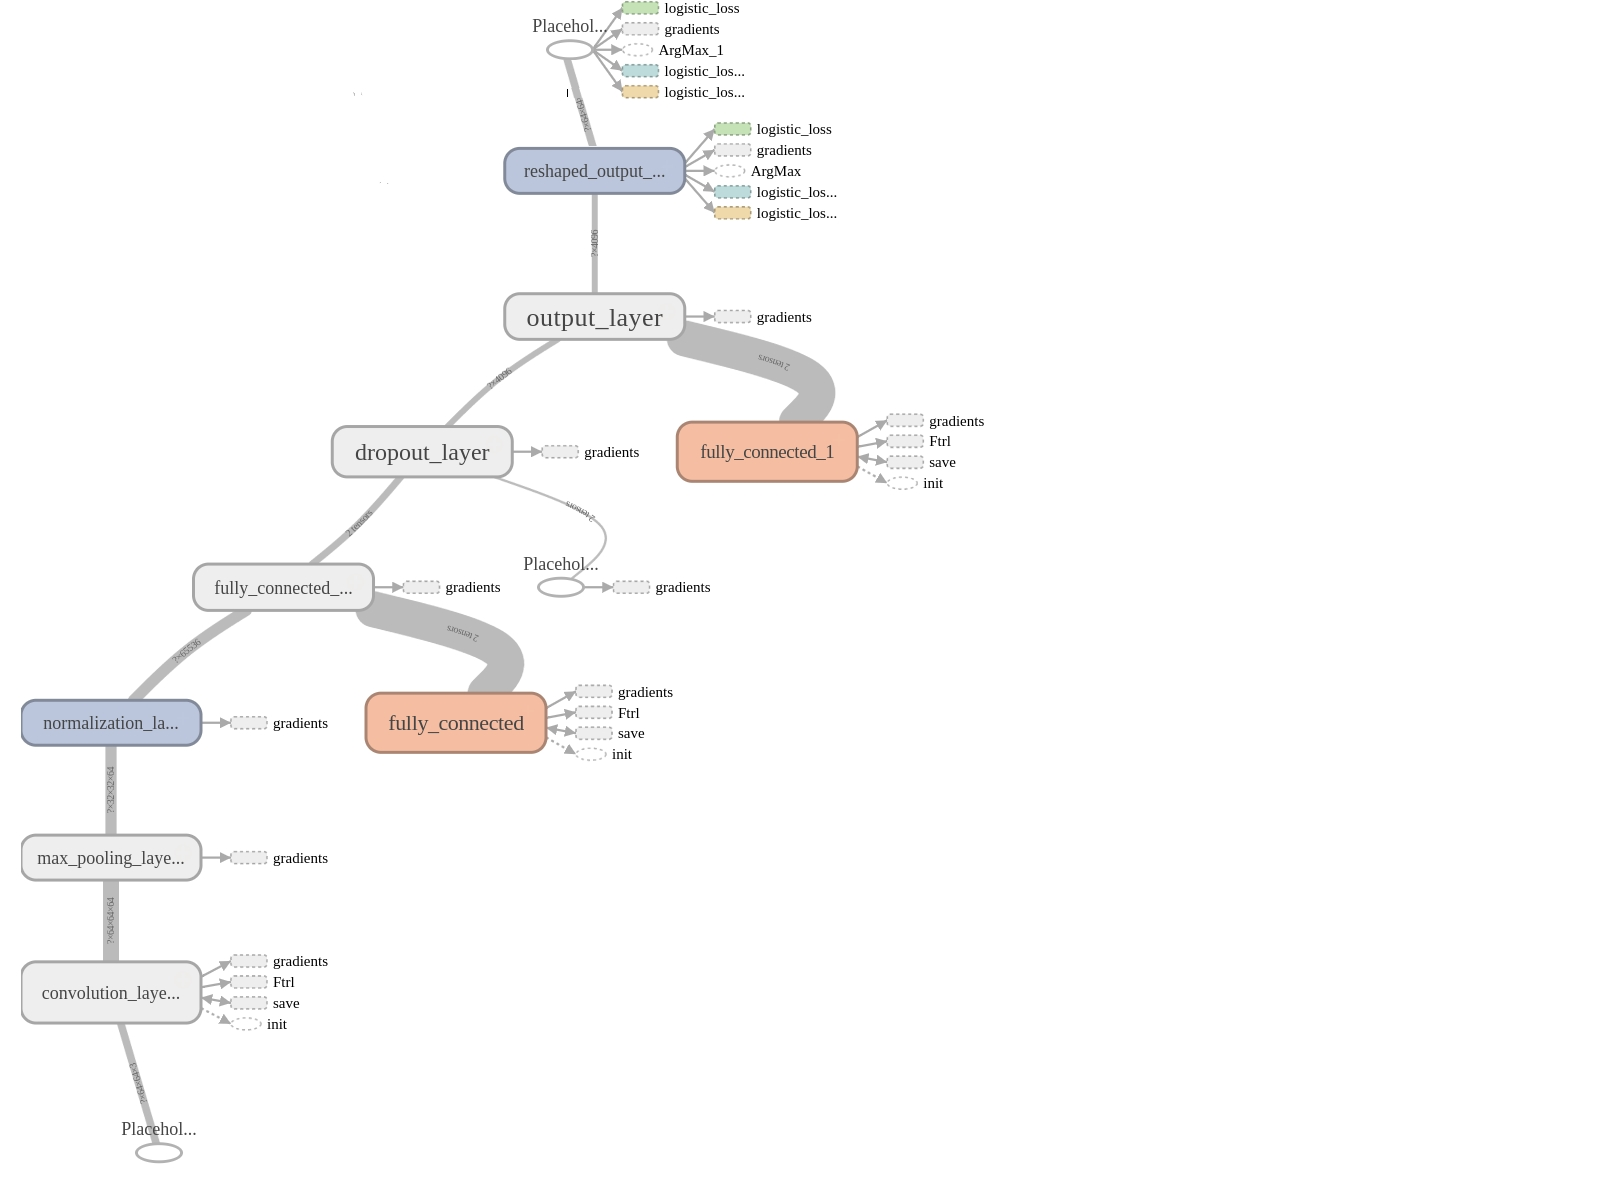
\includegraphics[scale=0.4]{graph-run.jpg}
		\caption[Návrh architektúry neurónovej siete]{
			Diagram reprezentujúci architektúru neurónovej siete, zdola vstupná konvolučná vrstva nasledovaná ostatnými vrstvami siete až po výstupnú, spolu s transformáciou na 2D maticu reprezentujúcu predikovanú mapu výraznosti pre vstupný obrázok
		}\label{my_tensorboard_cnn}
	\end{center}
\end{figure}

\subsection{Autoenkóder}
\label{autoencoder_design}
Ďalším z typov sietí, ktoré sme sa rozhodli otestovať je autoenkóder, konkrétne jeho variácia s konvolučnými vrstvami pre spracovanie obrazu. Jeho úloha je však trochu iná oproti klasickému čo najlepšiemu zrekonštruovaniu vstupu na výstupnej vrstve, miesto toho bude z enkódovaných (komprimovaných dát) predikovať mapy vizuálnej pozornosti. To dosiahneme použitím algoritmu učenia spätného šírenia chyby, kedy ako vstupné dáta budú sieti poskytnuté obrázky a očakávanými výstupmi budú práve mapy vizuálnej pozornosti.

Autoenkóder sa klasicky skladá z dvoch častí, prehľadná štruktúra je zobrazená na obrázku \ref{autoencoder_structure}. Prvou je enkóder, ktorý tvoria 3 konvolučné vrstvy, každá so svojou vlastnou vrstvou združovania, nasledované normalizačnou vrstvou a jednou plne prepojenou vrstvou (z angl. fully-connected layer). Konvolučné vrstvy majú každá filter o veľkosti \textit{3x3} a aktivačnú funkciu ReLU (popísaná v kapitole \ref{activation_functions}), vrstvy združovania podobne ako pri predchádzajúcom type siete používajú operáciu MAX s filtrom o veľkosti \textit{2x2} a krokom rovnako s veľkosťou \textit{2}. Cieľom týchto vrstiev je prakticky extrahovať relevantné črty a vstupný obrázok zmenšiť, resp. komprimovať, čo ďalej zabezpečuje spomínaná normalizačná a plne prepojená vrstva (bez aktivačných funkcií), ktorá už ale vstupný obrázok reprezentuje len ako komprimované jednorozmerné pole. 

Druhou časťou spomínaného autoenkóderu je tzv. dekodér, ktorý sa snaží prakticky zrkadlovými operáciami získať informácie z komprimovaných dát, vďaka čomu je schopný predikovať mapy vizuálnej pozornosti. Jeho vstupnou vrstvou je v podstate výstupná vrstva z enkóderu, ktorej tvar ale musí byť najprv zmenený pre nasledujúce konvolučné vrstvy. Tie sú dokopy štyri, prvé tri konvolučné vrstvy obsahujú filter s veľkosťou \textit{3x3} a aktivačnú funkciu ReLU. Každá z nich je ešte navyše nasledovaná vlastnou vrstvou
prevzorkovania (z angl. upsampling layer), ich cieľom je postupná rekonštrukcia do tvaru vstupného obrázku. Obsahujú vzorkovací faktor 2, na rozdiel od vrstiev združovania v enkóderi však miesto operácie MAX (ktorá dáta, resp. obrázok zmenší) duplikujú riadky a stĺpce poskytnutých dát (obrázka), vďaka čomu sa zväčší o vzorkovací faktor. Posledná výstupná konvolučná vrstva obsahuje filter s veľkosťou \textit{5x5} a aktivačnú funkciu sigmoid. Dáta na nej je ale ešte nutné pretransformovať na 2D maticu, reprezentujúcu nami požadovanú mapu výraznosti. Spomínané trénovanie pomocu algoritmu spätného šírenia chyby využíva Adadelta optimizér (popísaný v časti \ref{optimizers}).

\begin{figure}[H]
	\begin{center}
		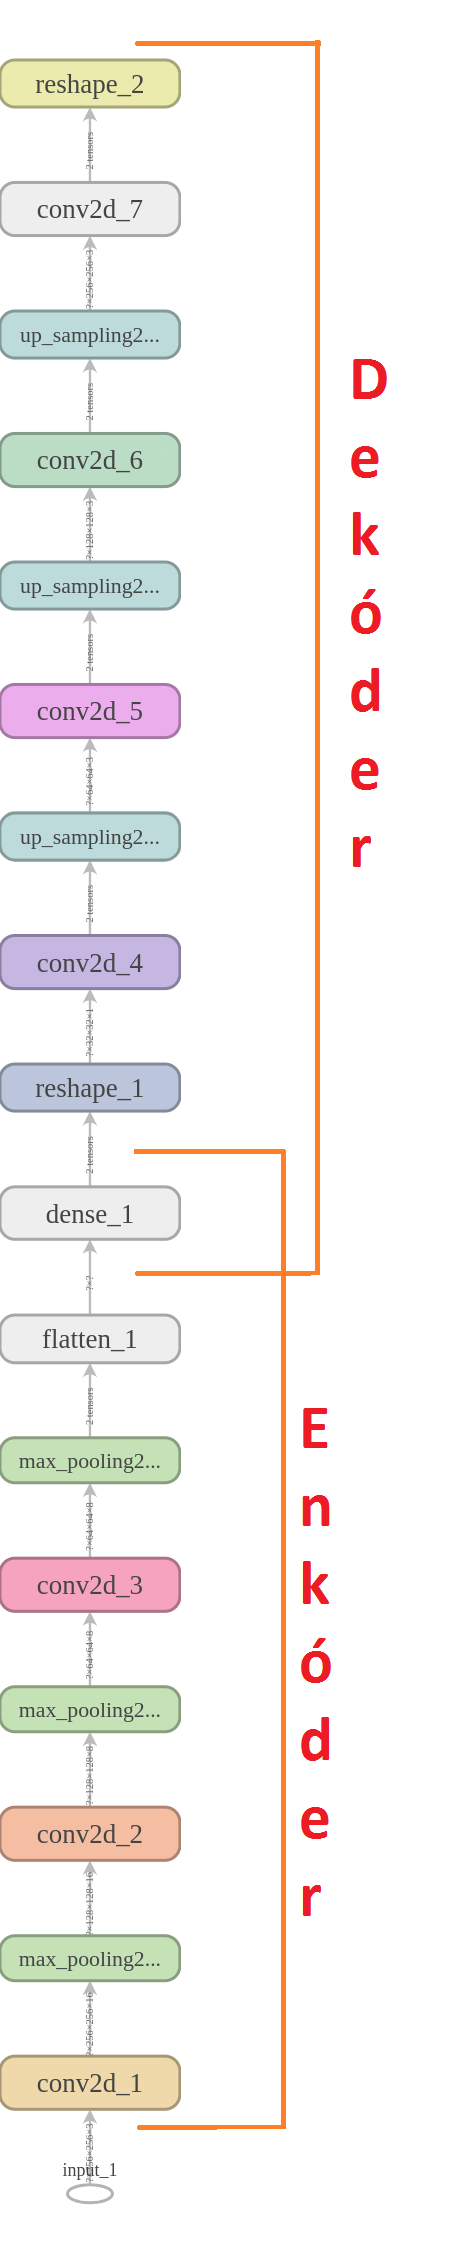
\includegraphics[scale=0.26]{enkoder-dekoder.png}
		\caption[Diagram navrhnutého autoenkóderu]{
			Diagram zobrazujúci architektúru autoenkóderu skladajúceho sa z dvoch častí - enkóderu a dekóderu. Postupne zdola prvá vstupná konvolučná vrstva nasledovaná ostatnými vyššie popísanými vrstvami enkóderu, potom dekóder so svojimi vrstami s konvolúciou a prevzorkovaním až napokon úplne hore výstupná vrstva s predikciou mapy vizuálnej výraznosti. 
		}\label{autoencoder_structure}
	\end{center}
\end{figure}

\subsection{Kombinácia VGG16 siete s autoenkóderom}
\label{vgg16_combination_with_autoencoder}
Pre experimentovanie so zapojením faktorov pozornosti zhora nadol sme navrhli sieť, ktorá kombinuje predikcie vyššie navrhnutého autoenkóderu s detekciou objektov VGG16 siete. Náčrt architektúry je na obrázku \ref{vgg_16_with_autoencoder}, podrobný diagram sa nachádza v prílohe \ref{vgg16_autoencoder_architecture_detailed}. 

Celá sieť je prakticky zložená z 3 častí:
\begin{itemize}
	\item enkóder - časť siete zodpovedná za detekciu salientných častí, je totožná s enkóderom v \ref{autoencoder_design} na obrázku \ref{autoencoder_structure}.
	\item VGG16 konvolučná časť - obsahuje prvých 10 konvolučný vrstiev VGG16 siete (diagram na obrázku \ref{vgg_net_model}) spolu s príslušnými vrstvami združovania (z angl. max pooling). Je zodpovedná za detekciu objektov. 
	\item dekóder - časť, v kt. sa postupne spájajú a upravujú predikcie z predošlých dvoch častí. Rovnako ako v návrhu z kapitoly \ref{autoencoder_design}, obsahuje štyri konvolučné vrstvy, prvá však nie je nasledovaná vrstvou prevzorkovania, ale vrstvou spájania - tá zabezpečuje spojenie predikcií z enkóderu a VGG16 konvolučnej časti. Po nej sú ďalej upravované pomocou ďalších dvoch konvolučných vrstiev nasledovaných vrstvou prevzorkovania, rovnako ako pri spomínanom predošlom návrhu. Tiež obsahujú aktivačnú funkciu ReLU a filter o veľkosti \textit{3x3}. Posledná výstupná konvolučná vrstva využíva filter s veľkosťou \textit{5x5} a aktivačnú funkciu sigmoid, nasledovaná je už len vrstvou, na ktorej sa dáta pretransformujú na 2D maticu reprezentujúcu predikovanú mapu výraznosti.
\end{itemize}

Pri trénovaní sme využili prenos učenia (popísaný v kapitole \ref{transfer_learning}), kedy vrstvy VGG16 konvolučnej časti boli už predtrénované k detekcii objektov. Počas trénovania celej siete sme potom experimentovali s vypnutím učenia pre spomínanú časť siete, keďže sme chceli zachovať kontext detekcie objektov. Samotné trénovanie prebiehalo pomocou algoritmu spätného šírenia chyby s použítím Adadelta optimizéru. 


\begin{figure}[H]
	\begin{center}
		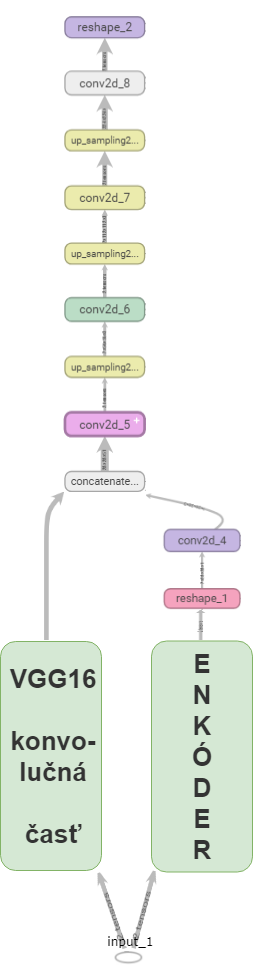
\includegraphics[scale=0.5]{vgg16_with_autoencoder.png}
		\caption[Náčrt architektúry VGG16 siete s autoenkóderom]{
			Náčrt architektúry VGG16 siete s autoenkóderom, VGG16 konvolučná časť obsahuje 10 konvolučných vrstiev pre detekciu objektov, enkóder je identický s enkóderom použitým v \ref{autoencoder_design}, podrobná architektúra je v prílohe \ref{vgg16_autoencoder_architecture_detailed}
		}\label{vgg_16_with_autoencoder}
	\end{center}
\end{figure}

